%
% Unless otherwise indicated, the copyright in this material is 
% owned by Joerg Evermann. This material is licensed to you under the 
% Creative Commons by-attribution non-commercial license (CC BY-NC 4.0)}
%
\section*{Learning Goals}

After reading this chapter, you should be able to:
\begin{itemize}
   \item Explain the importance of visually assessing data before predictive modelling.
   \item Build a linear regression model, including interaction effects and categorical predictors, and be able to assess its quality using cross-validation methods.
   \item Explain the goals and the differences between ridge regression, LASSO and Elasticnet
   \item Build regression models using different penalized linear regressions and evaluate their quality using cross-validation methods.
   \item Explain logistic regression and the purpose of the link function, including the concepts of log-odds or logits.
   \item Build a classification model using logistic regression and evaluate its quality using common metrics such as accuracy, and the ROC and AUC.
   \item Build a classification model using the KNN method and evaluate its quality using common metrics such as accuracy, and the ROC and AUC.
\end{itemize}

\section*{Sources and Further Reading}

The material in this chapter is based on the following sources. They are freely available. Consult them for additional information.

\begin{resourcebox}
Gareth James, Daniel Witten, Trevor Hastie and Robert Tibshirani: \emph{An Introduction to Statistical Learning with Applications in R}. 2nd edition, corrected printing, June 2023. (ISLR2) \\
\vspace{1mm}
\url{https://www.statlearning.com} \\
\vspace{1mm}
Chapters 2, 3, 4, 5
\end{resourcebox}

The book by James et al. provides an easy introduction to machine learning at the introductory undergraduate level. It focuses on applications, not mathematics, and contains many exercises using R. Concepts are well explained and illustrated. There is a similar book available by the same authors with applications in Python. This book is a more accessible of the following book.

\begin{resourcebox}
Trevor Hastie, Robert Tibshirani, and Jerome Friedman: \emph{The Elements of Statistical Learning}. 2nd edition, 12th corrected printing, 2017. (ESL) \\
\vspace{1mm}
\url{https://hastie.su.domains/ElemStatLearn/} \\
\vspace{1mm}
Chapters 2, 3, 4, 7
\end{resourcebox}

The book by Hastie et al. still sets the standard for statistical learning. It is widely used and cited. It's treatment is more technical than the previous book and there are no exercises in R or Python. However, it covers the concepts in more depth (and a few more formulas). However, it is still very accessible even to an undergraduate audience.

\begin{resourcebox}
Kevin P. Murphy: \emph{Probabilistic Machine Learning -- An Introduction}. MIT Press 2022. \\
\vspace{1mm}
\url{https://probml.github.io/pml-book/book1.html} \\
\vspace{1mm}
Chapters 4, 6, 9, 10, 11
\end{resourcebox}

Murphy's book is available under a creative-commons license. It is a somewhat more technical treatment of the material, but with many illustrations and examples. It is quite comprehensive in its coverage and targeted at the advanced undergraduate or graduate student. 

\section{Introduction}

This chapter is an introduction to supervised machine learning using R and includes both regression and classification problems. The chapter introduces linear regression and penalized regression models (ridge regression and LASSO). For classification, it introduces the methods of logistic regression and k-Nearest-Neighbours, which was already briefly discussed in the previous chapter. This chapter builds on the introductory material to supervised learning in the previous chapter. 

\section{Linear Regression}

Linear regression\index{Linear regression|see{Regression!linear}}\index{Regression!linear} fits a simple statistical model to a set of input and output variables. The true model is assumed to take the form:

\begin{align*}
f(X) &= Y = \beta_0 + \beta_1 X + \epsilon
\intertext{while the fitted, approximate model is:}
\hat{f}(X) &= \hat{Y} = \hat{\beta}_0 + \hat{\beta}_1 X
\end{align*}

The values of $\hat{f}(X) = \hat{Y}$ are called the \emph{fitted values}\index{Fitted values|see{Predicted values}} in statistics or the \emph{predicted values}\index{Predicted values} in machine learning. The difference in terminology reflects the fact that traditional statistics looks back at the training data for the output values determined by the model after it has been fit to the training data, whereas machine learning emphasizes prediction of output values for new inputs.

This equation shows the form of the assumed functional relationship between $X$ and $Y$ is linear in the parameters $\beta$. In other words, there are no polynomials or other transformations of $\beta$, such as $\beta_1^2$ or $\log \beta_1$. It is the linearity of the parameters that makes a regression linear, \emph{not} the linearity of the predictors. For example, adding a polynomial term $\beta_2 X^2$ to the right-hand side of this regression equation would still make this a linear regression. 

\begin{figure}
\centering

\includegraphics[width=.8\textwidth]{../class11/Figures_Chapters_1-6/Chapter3/3_1.pdf} \\

\scriptsize Source: ISLR2 Figure 3.1
\caption{A linear regression model}
\label{fig:regression_chap12}
\end{figure}

Figure~\ref{fig:regression_chap12} shows the fitted regression line expressed by the intercept ($\hat{\beta}_0$) and slope ($\hat{\beta}_1$) parameters. The distance between this line and the data points (coloured red) represents the error term $\epsilon$ in the regression equation. Importantly, the error is the vertical differences in the $Y$ direction between fitted regression line and the data point, \emph{not} the shortest distance between the regression line and the data point. 

The first task in performing a regression analysis is to identify the form of the regression model or regression equation. While Figure~\ref{fig:regression_chap12} fitted a model that is linear in $X$, it is clear that this model is not a good fit for small $X$ values, as the corresponding observations are all below the regression line. 

To identify an appropriate functional form, it is insufficient to simply examine summary statistics like correlations or covariances between variables. Figure~\ref{fig:datasaurus} shows twelve data sets with the same correlation between the two variables. It is clear that none of them can be fitted to a simple moodel that is linear in $X$. While some, like the circle or the bullseye data set, can be appropriately transformed and fitted to linear regression models that involve polynomials or other functions of $X$, it is not clear what functional form the dinosaur head might take.

\begin{figure}
\centering
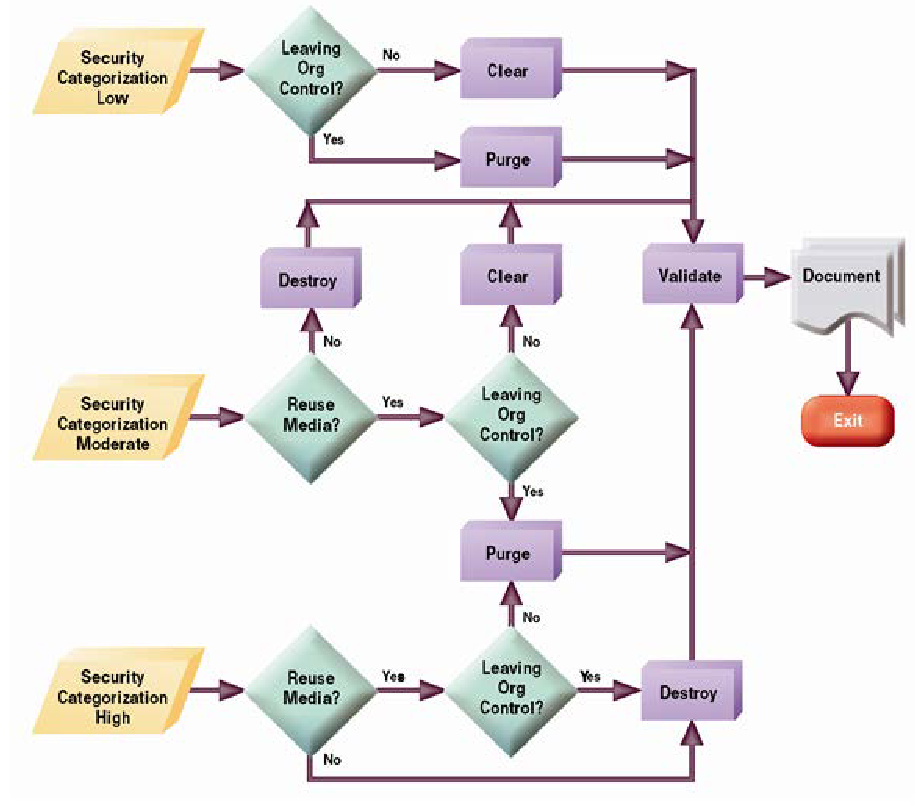
\includegraphics[width=.85\textwidth]{screen1.png} \\

\scriptsize Source: Murphy Figure 2.6 \\ \vspace{3mm}
\normalsize
\caption[The ''Datasaurus Dozen'' data sets]{The ''Datasaurus Dozen'' -- All datasets have the same correlation between the two variables}
\label{fig:datasaurus}
\end{figure}

It is also insufficient to fit a model that is linear in $X$ and use the fit as indication for the appropriateness of the model. Consider the data sets shown in Figure~\ref{fig:murphy31}. The correlations between the two variables are shown above each data set. Visual inspection is sufficient to show that data sets with the same correlation do not necessarily have the same regression slope, or should even be fitted to the same linear model. 

\begin{figure}
\centering
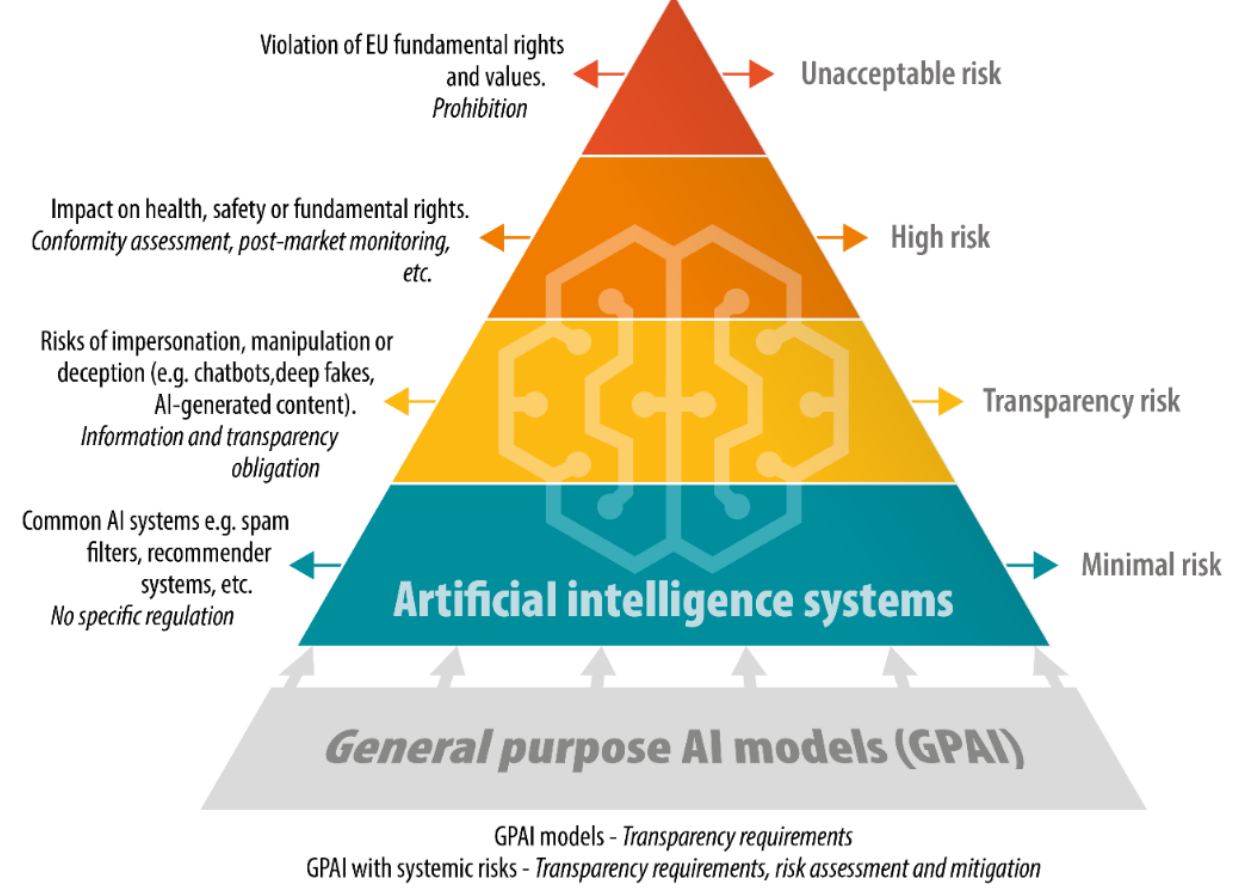
\includegraphics[width=.9\textwidth]{screen2.png} \\

\scriptsize Source: Murphy Figure 3.1 \\ \vspace{3mm}
\normalsize
\caption[Correlation and regression slopes]{Datasets with the same correlation (as indicated above each dataset) between two variables do not need to have the same regression slope}
\label{fig:murphy31}
\end{figure}

The objective for estimating the parameters $\beta_0$ and $\beta_1$ from the data set is to minimize the residual or error, that is, the difference between $f$ and $\hat{f}$. So that positive and negative differences do not compensate for each other, the difference is either squared or the absolute value is taken. The former is called \emph{mean squared error} (MSE) while the latter is called \emph{mean absolute error} (MAE). In statistics, a closely related concept is the \emph{residual sum of squares} (RSS). The MSE is the RSS divided by the number of observations $n$, and minimizing one also minimizes the other\index{Residual sum of squares}\index{RSS|see{Residual sum of squares}}. While the discussion in the previous chapter indicated that the MAE is more robust in that outliers, i.e. observations with large errors, have less influence on the estimated values of the parameters, it is customary to fit linear regression models using the RSS or the MSE.

\begin{align*}
RSS &= \sum_i \left( y_i - \hat{\beta}_0 - \hat{\beta}_1 x_i \right)^2 \\
MSE &= \frac{1}{n} RSS
\end{align*}

The linear regression model is simple enough that an optimal solution can be derived analytically. The optimal least-squares estimates are:

\begin{align*}
\hat{\beta}_1 &= \frac{\sum_i (x_i - \bar{x})(y_i - \bar{y})} {\sum_i (x_i - \bar{x})^2} \\
\hat{\beta}_0 &= \bar{y} - \hat{\beta}_1 \bar{x}
\end{align*}
\noindent where $\bar{x}$ and $\bar{y}$ are the sample means.

%The parameter value estimates have \emph{standard errors} associated with them that indicate the uncertainty of these estimates. This is based on the idea that the training data set is a small random sample from the overall population, and taking other random samples may well yield slightly different parameter values. 

%Using the standard errors of the estimates, a \emph{t statistic}\index{t-test} can be calculated from the difference of the estimate of a parameter $\hat{beta}$ and some value $V$.

%\begin{align*}
%t = \frac{\hat{\beta} - V}{SE(\hat{\beta})}
%\end{align*}

%The statistic $t$ is a random variable whose values are distributed according to a student-t probability distribution. This allows one to calculate the probability of observing a value of $t$ or larger under the assumption that $\hat{\beta} = V$, that is, there is no difference between $V$ and the estimate of the parameter $\hat{\beta}$. If the calculated probabily is very small, it is unlikely that this assumption holds and one might conclude that $\hat{\beta} \neq V$. This procedure is called the \emph{t-test}. In most applications of this test to regression model parameters, $V$ is set to $0$. Because for large sample sizes the student-t distribution approaches the normal (Gaussian) probability distribution, the probability is sometimes calculated from this distribution, the statistic is called the $z$ statistic and the test is then called a \emph{z-test}.

An important statistic in linear regression analysis is the proportion of explained variance, designated as $R^2$. It is defined as:

\begin{align*}
R^2 = \frac{TSS - RSS}{TSS} = 1 - \frac{RSS}{TSS}
\end{align*}

\noindent where $TSS = \sum_i(y_i - \bar{y})^2$ is the total sum of squares. An $R^2$ value close to $1$ indicates that the fitted regression model explains a large proportion of the variability in the data set, that is, it explains the data well. In contrast, a value close to $0$ indicates that the fitted regression model explains very little of the observed variability, it does not explain the observed data well. Another important interpretation of the $R^2$ is as the squared correlation between the true $Y$ and the fitted or predicted values $\hat{Y}$. In this interpretation too, a value close to one indicates predicted values closely correlated with the true values, that is, a good model, whereas a low value indicates they are not closely correlated, that is, a bad model.

Adding additional predictors into the linear regression model is straightforward, as is the inclusion of qualitative or categorical predictors. For example, a model with two predictors $X_1$ and $X_2$ assumes the true form

\begin{align*}
Y = \beta_0 + \beta_1 X_1 + \beta_2 X_2 + \epsilon
\end{align*}

\noindent and fits a plane to a set of points in three dimensional ($X_1, X_2, Y$) space, as shown in Figure~\ref{fig:plane}. 

\begin{figure}
\centering
\includegraphics[width=.66\textwidth]{../class11/Figures_Chapters_1-6/Chapter3/3_4.pdf}  \\

\scriptsize Source: ISLR2 Figure 3.4
\caption{Example linear regression with two predictors}
\label{fig:plane}
\end{figure}

Qualitative predictors (called \emph{factors} in statistics)\index{Factor} wich multiple, exclusive \emph{levels}\index{Factor level} or categories can be included using \emph{dummy variables}\index{Dummy variable}. A categorical variable that can take on $k$ values requires $k-1$ binary dummy variables. For example, a factor $x$ that has four levels ''a'', ''b'', ''c'', and ''d'' might be encoded using three dummy variables as follows:

\begin{align*}
x_{i1} = \begin{cases}
1 & \text{level ''a''} \\
0 & \text{else}
\end{cases} \\
x_{i2} = \begin{cases}
1 & \text{level ''b''} \\
0 & \text{else}
\end{cases} \\
x_{i3} = \begin{cases}
1 & \text{level ''c''} \\
0 & \text{else}
\end{cases}
\end{align*}

\noindent Note that $x_{i1} = x_{i2} = x_{i3} = 0$ represents level ''d''. Such \emph{contrasts}\index{Contrast (for categorical predictor)} determine how factor levels are coded using dummy variables.

Earlier, it was noted that a linear model is linear in its parameters, not necessarily in its input variables. Hence, it is possible to include transformations of input variables in a linear regression model, such as polynomials, products, or other functional transformations like logarithms, square roots, etc. For example, the model

\begin{align*}
Y = \beta_0 + \beta_1 X_1 + \beta_2 X_1^2 + \beta_3 X_2 + \beta_4 X_1 X_2 + \epsilon
\end{align*}

\noindent is still linear in its parameters $\beta_i$. This model also shows the difference between \emph{input variables} and \emph{predictors} or \emph{features} that was alluded to in the previous chater. This model has two input variables $X_1$ and $X_2$ but has four predictors or features, $X_1$, $X_1^2$, $X_2$, and $X_1 X_2$. In statistics terminology, the coefficients of single input variables, here $\beta_1$ and $\beta_3$, are said to represent \emph{main effects}\index{Main effect}, while the parameters of products of two or more input variables, here $\beta_4$ are said to represent \emph{interaction effects}{Interaction effect}. Interaction effects can include the product of a numerical variable and a dummy binary variable. This results in different regression slopes for different categories or factor levels, as shown in the example in Figure~\ref{fig:groupinteraction} where the left panel shows no interaction effect, that is, the lines are parallel with the same slopes. The right panel shows an interaction effect where the slopes for different categories are different.

\begin{figure}
\centering
\includegraphics[width=.9\textwidth]{../class11/Figures_Chapters_1-6/Chapter3/3_7.pdf} \\

\scriptsize Source: ISLR2 Figure 3.7
\caption{Example interaction effect in linear regression}
\label{fig:groupinteraction}
\end{figure}

An example of polynomial predictors like $X^2$, $X^3$ or higher degrees is shown in Figure~\ref{fig:polynomial_chap12}. As the figure shows, and as is true in general, increasing the number of predictors increases the flexibility of the model to fit the data. This results in smaller model bias but usually at the expense of model variance. 

\begin{figure}
\centering

\includegraphics[width=.8\textwidth]{../class11/Figures_Chapters_1-6/Chapter3/3_8.pdf} \\

\scriptsize Source: ISLR2 Figure 3.8
\caption{Regression example with polynomial predictors}
\label{fig:polynomial_chap12}
\end{figure}


\FloatBarrier
\section{Linear Regression in R}

Linear regression is part of the basic R system, no libraries need to be installed. The function \texttt{lm()} requires a formula representing the regression model and a data frame, and returns a linear model. 

The following example uses the \texttt{Boston} data set that contains housing prices (''median value'', \texttt{medv}) as well as demographic and socioeconomic information for suburbs in the city of Boston. The data is available as part of the \texttt{ISRL2} package\footnote{The R code for this example is based on material in Section 3.6 of ISLR2}.

First, examine the data, get summary statistics, examine the first few rows of the data frame, and create scatterplots to identify the form of a linear model:

\begin{Rcode}
# Data set from the textbook 'Introduction to 
# Statistical Learning with Applications in R'
library(ISLR2)

# Get a description of the data
?Boston

# Get a summary and examine first few rows
summary(Boston)
head(Boston)

# Bivariate scatterplots
plot(Boston)
\end{Rcode}

The formula interface to \texttt{lm()} is the easiest to use and resembles the way one would write the regression equation. The $\sim$ sign separates the output on the left side from the predictors or features on the right side of the formula. A \texttt{1} in the formula represents the intercept ($\beta_0$ in the formula above). The intercept is normally added automatically but can be explicitly added or removed (using \texttt{-1}) as needed. 

The following R code fits a simple model to predict the median house value, shows the model summary and produces a scatterplot with the fitted model regression line running through it. 

\begin{Rcode}
# Fit a model with intercept only
fitted.model <- lm(medv ~ 1, data=Boston)
summary(fitted.model)

# Fit a model with predictor lstat
fitted.model <- lm(medv ~ lstat, data=Boston)
summary(fitted.model)

# Plot the data and the regression line
plot(medv ~ lstat, data=Boston)
abline(fitted.model, lwd=3, col='red')
\end{Rcode}

The \texttt{predict()} function is used to predict new values, given a fitted model and an optional data frame of predictor values, that is, it computes $\hat{y}$. When no predictor values are provided, the function predicts from the data set it was trained on. The \texttt{residuals()} function computes the difference between true and fitted values, that is, it computes $y - \hat{y}$.

\begin{Rcode}
For training data
y.hat <- predict(fitted.model, Boston)
# For new data
newData <- data.frame(lstat = c(5, 10, 15))
predict(fitted.model, newData)

# Plot the residuals against predicted values
plot(predict(fitted.model), residuals(fitted.model))
\end{Rcode}

The following R code fragment adds a second input variable (age) to the model. It also demonstrates some special notation in the R formula interface, such as the \texttt{.} to include all main effects, the \texttt{:} to specify interaction effects, and the \texttt{*} to include both main and interaction effects.

\begin{Rcode}
# Add another predictor
fitted.model <- lm(medv ~ lstat + age, data=Boston)

# Add all main effects
fitted.model <- lm(medv ~ ., data=Boston)

# Add interaction terms
fitted.model <- lm(medv ~ lstat + age + lstat:age, data=Boston)
   
# Shorter and equivalent
fitted.model <- lm(medv ~ lstat*age, data=Boston)
summary(fitted.model)
\end{Rcode}

The next example adds polynomial terms to the regression. It uses the \texttt{I(.)} function in R that can also be used with other transformations of the inputs, such as \texttt{I(sqrt(.))} or \texttt{I(log(.))}. To make it easier to include all polynomials up to a particular degree, one can us the \texttt{poly(.)} function:

\begin{Rcode}
# Add a polynomial term; use the I(.) function
# for any data transformations, such as log(),
# or exp() or sqrt() as well as polynomials
fitted.model <- lm(medv ~ lstat + I(lstat^2), data=Boston)
summary(fitted.model)

# Add all polynomial terms up to degree 5
fitted.model <- lm(medv ~ poly(lstat, 5), data=Boston)

# Note the coefficients for the polynomials in the summary
summary(fitted.model)
\end{Rcode}

The use of categorical input variables is illustrated in the following example that uses the \texttt{Carseats} data, also from the \texttt{ISLR2} package. The data frame represents sales data of car seats for different stores and a range of store characteristics in other variables, many of which are categorical. 

The following R code demonstrates functions for dealing with categorical variables, called ''factors'' in R. The example then fits a regression model to predict Sales from the the main effects of all input variables in the data frame.

\begin{Rcode}
?Carseats

# Identify factor/categorical variables and their levels:
is.factor(Carseats$ShelveLoc)
levels(Carseats$ShelveLoc)
levels(Carseats$Urban)
levels(Carseats$US)

# Contrasts show the dummy variables created (columns) and 
# the values they take for different  factor levels (row)
contrasts(Carseats$ShelveLoc)
contrasts(Carseats$US)

# Fit the model
summary(lm(Sales ~ . , data=Carseats))
\end{Rcode}

\begin{exercisebox}
\noindent Use the \texttt{Auto} data set from the ISLR2 library with \texttt{mpg} as the target.
  \begin{enumerate}
     \item Perform a linear regression with \texttt{horsepower} as predictor
     \item Is there a relationship between the predictor and target? What form and how strong?
     \item What is the predicted \texttt{mpg} value for a \texttt{horsepower} of 98? 
     \item Plot the response and predictor. Use the \texttt{abline()} function to add the regression line
     \item Produce a scatterplot of all variables
     \item Perform a linear regression of all main effects (except for the variable \texttt{name}).
     \item Use the \texttt{*} and \texttt{:} symbols to add interaction effects.
     \item Add transformations of the predictors (using the \texttt{I(.)} function) such as $\log(X)$, $\sqrt{X}$, $X^2$.
  \end{enumerate}

{\footnotesize \vspace{\baselineskip} Source: ISLR2 Section 3.7}
\end{exercisebox}

\begin{exercisebox}
\noindent Use the \texttt{Carseats} data set from the ISLR2 library with \texttt{Sales} as the target.
  \begin{enumerate}
     \item Perform a linear regression with \texttt{Price}, \texttt{Urban} and \texttt{US} as predictors
     \item Interpret the coefficients. Tip: Some variables are categorical
     \item Remove non-significant predictors
     \item How well do the two models fit the data in terms of their $R^2$?
  \end{enumerate}

{\footnotesize \vspace{\baselineskip} Source: ISLR2 Section 3.7}
\end{exercisebox}

\section{Cross-Validation in R}

The previous chapter already introduced the concepts of cross-validation. Recall that the appropriate way to judge the predictive performance of a model is not to evaluate it on its training data, but to evaluate it on unseen test data. This section illustrates three different cross-validation approaches in R, beginning with the validation set or holdout sample approach, which splits the data set randomly into training and test data. 

The following example uses the \texttt{Auto} data set from the \texttt{ISLR2} package, which contains information on different vehicle models, their fuel economy (''miles per gallon'', mpg) and vehicle characteristics\footnote{The R code for this example is based on material in Section 5.3 of ISLR2}.

Randomly splitting the data set is accomplished using the \texttt{sample()} function in R which returns a boolean vector with values \texttt{TRUE} or \texttt{FALSE} that can be used to select the appropriate data from the data frame. 

To make the example repeatable, the initial seed of the pseudo-random number generator (RNG)\index{Random number generator}\index{RNG|see{Random number generator}} is set to a fixed value with \texttt{set.seed()}. Computers cannot generate truly random number; they are deterministic machines. The pseudo-random numbers they generate are computed by a deterministic algorithm, the ''random number generator'' (RNG), based on a given start value. With the same start value, the algorithm produces the same sequence of numbers. A good RNG produces numbers that are effectively indistinguishable from true trandom numbers.

\begin{Rcode}
# Set the seed for the pseudo-random number generator (RNG)
set.seed(1)

# Randomly use half the Auto data as training sample
train.idx <- sample(nrow(Auto), nrow(Auto)/2)
train.data <- Auto[train.idx,]
test.data <- Auto[-train.idx,]

# Fit model to (train model on) a subset
fitted.model <- lm(mpg ~ horsepower, data=train.data)

# Calculate the training MSE by predicting from the training data set
mean((train.data$mpg - predict(fitted.model, train.data))^2)

# Calculate the test data MSE by predicting from the test data set
mean((test.data$mpg - predict(fitted.model, test.data))^2)

# The MSE can also be calculated from the squared residuals
mean(summary(fitted.model)$residuals^2)
\end{Rcode}

The next R code block illustrates Leave-One-Out Cross-Validation (LOOCV), where one observation is used as test observation, and the remainder form the training data. This is repeated so that each observation becomes the test observation in turn. The errors are then averaged. 

While this can be done manually in R using an iteration over the data frame, the library \texttt{boot} provides easy-to-use cross-validation functions for models fitted using the \texttt{glm()} function (generalized linear models). Note that LOOCV is just k-fold cross-validation where $k$, the number of test data folds, is equal to the number of observations.

\begin{Rcode}
library(boot)

# Fit a model with glm and show its summary
fitted.model <- glm(mpg ~ horsepower, data=Auto)
summary(fitted.model)

# LOOCV is k-fold CV where k equals the number of observations
cv.err <- cv.glm(Auto, fitted.model, K=nrow(Auto))
cv.err$delta[1]
\end{Rcode}

The same functions can be used for k-fold CV with a typical value for $k$:

\begin{Rcode}
cv.err <- cv.glm(Auto, glm.fit, K=10)
cv.err$delta[1]
\end{Rcode}

Cross-validation is useful for comparing different models, as shown in the following example that fits linear regression models with different degrees of polynomials to a data frame and computes their cross-validation errors using a \texttt{for} loop in R:

\begin{Rcode}
set.seed(1)
cv.err <- rep(0, 5)
for(i in 1:10) {
  fitted.model <- glm(mpg ~ poly(horsepower,i), data=Auto)
  cv.err[i] <- cv.glm(Auto, fitted.model, K=10)$delta[1]
}
print(cv.err)
\end{Rcode}

\begin{exercisebox}
\begin{enumerate}
  \item Fit a regression model to the \texttt{Boston} data set with \texttt{medv} as target, and \texttt{age}, \texttt{lstat}, and \texttt{ptratio} as predictors
  \item Using the holdout approach, compute the test error of this model. Perform the following steps
  \begin{enumerate}
     \item Split the data set using 75\% for training and 25\% for testing
     \item Fit the model to training data
     \item Predict the target for the testing data
     \item Compute the test error
  \end{enumerate}
  \item Repeat the previous step 2 times, using different splits. How do the results change?
  \item Calculate the mean and the variance of the test errors of the four splits. 
  \item Calculate the test error estimate using LOOCV. Compare your result to the mean that you computed in step 4.
  \item Calculate the test error estimate using 10-fold cross-validation. Compare the estimate to the mean that you computed in step 4
\end{enumerate}
\end{exercisebox}

\section{Shrinkage Methods}

Shrinkage methods are so-called because their aim is shrink the magnitude of the regression parameter values $\hat{\beta}_i$. This is primarily to avoid overfitting a model to one specific data set. In other words, they are a kind of \emph{regularization}, that is, a type of method to avoid or prevent overfitting of models. Shrinkage methods for linear regression model works by \emph{penalizing} the model for large regression parameter values, that is, by performing \emph{penalized regression}\index{Shrinkage methods}\index{Penalized regression|see{Shrinkage methods}}\index{Regularization}. There are three frequently used types of penalized regression or linear regression regularization: L1 regularization penalizes large absolute parameter values (that is, the L1 norm of the vector of parameters $\hat{\beta}$), L2 regularization penalizes large squared parameter values (that is, the L2 norm of the vector of parameters $\hat{\beta}$, and Elastic Net regularization is a combination of both. L1 regularization is also known as the \emph{LASSO} (''least absolute shrinkage and selection operator'') while L2 regularization is known as \emph{ridge regression} or Tikhonov regularization. 

\subsection{Ridge Regression}

The loss function or minimization objective of ridge regression\index{Ridge regression}\index{L1 regularization|see{Ridge regression}} is the usual RSS that now also includes a term that penalizes large values of $\beta$. 

\begin{align*}
\text{Minimize} \quad RSS + \lambda \sum_{j=1}^p \beta_j^2 = RSS + \lambda ||\beta||_2^2
\end{align*}

\noindent where $||\cdot||_2$ indicates the \emph{L2 vector norm}, that is, the sum of squared entries of the vector $\beta$. 

Because the scale, that is, the standard deviation or variance, of different predictors affects the size of their associated $\beta$ parameter values, \emph{all predictors should be rescaled or standardized to have the same standard deviation prior to performing a ridge regression}. 

The degree of penalization or the amount of shrinkage is controlled by the parameter $\lambda$. Larger values for $\lambda$ increase the penalty, thus generally leading to larger model bias but smaller variance. This effect is shown in Figure~\ref{fig:ridgebias} where the left panel shows the bias (black line), the variance (turquoise line) and the total MSE (pink line) as a function of $\lambda$ and the right panel shows the bias, the variance, and the total MSE as a function of the proportion to which the L2 norm of the $\beta$ is restricted or penalized compared to the unrestricted estimates, i.e. $||\hat{\beta}^R_\lambda||_2 / ||\hat{\beta}||_2$ where $||\cdot||_2$ indicates the \emph{L2 vector norm}, i.e. the sum of the squared elements of the vector.

\begin{figure}
\centering
\includegraphics[width=.9\textwidth]{../class11/Figures_Chapters_1-6/Chapter6/6_5.pdf}

\scriptsize Source: ISLR2 Figure 6.5 \normalsize \\

\caption[Bias, variance, and MSE in ridge regression]{Bias (black), variance (turquoise), and MSE (pink) in ridge regression}
\label{fig:ridgebias}
\end{figure}

Figure~\ref{fig:ridgemultiple} shows this effect for a polynomial of degree 14 that is fitted to data set of 21 observations. The different panels show different degrees of penalization or shrinkage as indciated by different values of $\lambda$. The bottom right panel in Figure~\ref{fig:ridgemultiple} shows the MSE on the training data (blue) and test data (red) for multiple values of $\lambda$. It is clear that the unpenalized model in panel (a) of Figure~\ref{fig:ridgemultiple} overfits, while models that are penalized too heavily underfit and have large bias, such as the model in panel (c) of Figure~\ref{fig:ridgemultiple}. 

\begin{figure}
\centering
\includegraphics[width=0.9\textwidth]{screen4.png}\\
\scriptsize Source: Murphy Figure 4.5

\caption{Fitting a degree 14 polynomial with ridge regression}
\label{fig:ridgemultiple}
\end{figure}

\subsection{LASSO}

In contrast to the ridge regression, where the model parameter values are shrunk towards zero, but are never forced to equal zero, the LASSO does just that. In this form of penalized regression, as the degree of penalty is increased, model parameter values are set to 0, effectively making the LASSO a model selection method or \emph{predictor selection method} as well, that is, it can be used to select only important predictors. This is reflected in its name: ''Least Absolute Shrinkage and Selection Operator''. The advantage over ridge regression is that this results in more parsminious, that is, smaller, models that are easier to interpret.

The loss function or minimization objective of the LASSO\index{Least absolute shrinkage and selection operator}\index{LASSO|see{Least absolute shrinkage and selection operator}}\index{L2 regularization|see{Least absolute shrinkage and selection operator}} is the RSS but penalized for the L1 norm of the vector of parameters $\beta$. As in ridge regression, the amount of shrinkage is controlled by a parameter $\lambda$.

\begin{align*}
\text{Minimize} \quad RSS + \lambda \sum_{j=1}^p |\beta_j| = RSS + \lambda ||\beta||_1
\end{align*}

\noindent where $||\dot||_1$ indicates the \emph{L1 vector norm}, that is the sum of the absolute values of the elements of the vector $\beta$.

\begin{figure}
\centering
\includegraphics[width=.85\textwidth]{../class11/Figures_Chapters_1-6/Chapter6/6_6.pdf} \\

\scriptsize Source: ISLR2 Figure 6.6
\caption{Preditor selection in the LASSO}
\label{fig:lasso1}
\end{figure}

The model selection property of the LASSO are shown in Figure~ref{fig:lasso1}. The left panel shows the value of different model parameters as a function of the penalization parameter $\lambda$. As $\lambda$ increases, fewer and fewer parameters are allowed to retain absolute values larger than 0. The same is shown in the right panel of Figure~\ref{fig:lasso1}, but now as a function of the relative size of the restricted L1 norm of $\beta$ compared to the L1 norm of the unconstrained $\beta$.

The LASSO and ridge regression shrinkage or penalty parameter $\lambda$ is typically chosen through cross-validation to minimize the cross-validation or test error. For cross-validation, a ''grid'' or range of possible values of $\lambda$ is defined. A model is fitted for each value of $\lambda$ and its cross-validation or test error is calculated. The final model is then fitted using the optimal value of $\lambda$, that is, the value that results in the lowest cross-validation or test error.

\begin{figure}
\centering
\includegraphics[width=.85\textwidth]{../class11/Figures_Chapters_1-6/Chapter6/6_13.pdf} \\

\scriptsize Source: ISLR2 Figure 6.13
\caption{Cross-validation error in the LASSO}
\label{fig:lasso2}
\end{figure}

This is illustrated in Figure~\ref{fig:lasso2} for a LASSO, where the left panel shows the cross-validation error as a function of the relative shrinkage. Towards the left of the graph in that panel, where shrinkage is maximal, the model underfits, resulting in a relative large error due to a large bias, whereas to the right of the graph, where shrinkage is minimal, the model overfits, leading to a large cross-validation error due to large variance. The right panel of Figure~\ref{fig:lasso2} shows the size of model parameter values; at the optimal $\lambda$ only two model parameters are different from zero, that is, only two predictors are selected for the model. 

\subsection{Elastic Net}

The Elactic Net\index{Elastic net} is a combination of rigde regression and LASSO, controlled by the parameter $\alpha$. The Elastic Net penalty is defined as

\begin{align*}
\lambda \left( \alpha ||\beta||_1  + (1-\alpha)||\beta||_2^2 \right)
\end{align*}

When $\alpha=0$ the Elastic Net reduces to a ridge regression, and for $\alpha=1$ the Elastic Net reduces to the LASSO. The optimal combination of $\alpha$ and $\lambda$ is found through cross-validation as described above.


\section{Shrinkage Methods in R}

The \texttt{glmnet} library for R implements the Elastic Net which can be used for both ridge regression and LASSO as well, simply by choosing the appropriate value for the parameter $\alpha$.

The following R code examples use the \texttt{Hitters} data set containing information on baseball players. The data set is part of the \texttt{ISLR2} library. The code examples model a player's Salary as the output or prediction target and use a number of other variables as inputs\footnote{The R code for this example is based on material in Section 6.5.2 of ISLR2}. 

\begin{Rcode}
library(ISLR2)
library(glmnet)

# Remove missing values
Hitters <- na.omit(ISLR2::Hitters)
\end{Rcode}

The \texttt{glmnet(.)} function requires separate $x$ (predicots) and $y$  (target) values, instead of providing a formula interface like the \texttt{lm(.)} and \texttt{glm(.)} functions. To create dummy variables for categorical variables, use the \texttt{model.matrix} function:

\begin{Rcode}
# Create dummy variables for categorical variables
# and remove the intercept (first column) from the model
x <- model.matrix(Salary ~ ., Hitters)[, -1]
y <- Hitters$Salary
\end{Rcode}

\noindent To illustrate the concepts of ridge regression, the following R code fits a ridge regression model with $\lambda=10$ using the \texttt{glmnet()} function with $\alpha=0$. This value of $\alpha$ indicates ridge regression, that is only penalization of the L2 norm. 


\begin{Rcode}
# Fit the model
ridge.model <- glmnet(x, y, alpha=0, lambda=10)

# Examine coefficients:
coef(ridge.model)

# Examine L2 norm (penalty to RSS) (without intercept)
L2.norm = sqrt(sum(coef(ridge.model)[-1]^2))

# Examine MSE:
mean((y-predict(ridge.model, x))^2)
\end{Rcode}

The optimal value for $\lambda$ is chosen through cross-validation. For this, a holdout test data set is created to evaluate the final model. The training data set portion is used with cross-validation, so that the final model evaluation is done on an independent data set from model selection. 

\begin{Rcode}
# Randomly split the Hitters data
train.idx <- sample(nrow(Hitters), nrow(Hitters)/2)
x.train <- x[ train.idx,]
x.test  <- x[-train.idx,]
y.train <- y[ train.idx]
y.test  <- y[-train.idx]
\end{Rcode}

\noindent The \texttt{glmnet} library provides the function \texttt{cv.glmnet} as an easy-to-use way to combine Elastic Net model fitting with k-fold cross-validation. The following example uses 5-fold CV on the training portion of the data set:

\begin{Rcode}
# 5-fold cross-valiation, use MSE as metric
cv.out <- cv.glmnet(x.train, y.train, alpha=0, 
                    nfolds=5, type.measure='mse')
\end{Rcode}

The next R code block shows the optimal $\lambda$ and plots the MSE for different values of $\lambda$. The generated plot is shown in Figure~\ref{fig:glmnetcv}. It includes the standard errors of the MSE (as determined by cross-validation) and the number of non-zero coefficients (indicated above the graph). The left vertical line indicates the optimal $\lambda$, while the right vertical line indicates that largest $\lambda$ for which the MSE is within one standard error of the minimum MSE, that is, of the MSE of the optimal $\lambda$.

\begin{Rcode}
print(cv.out)
plot(cv.out)
lambda.opt <- cv.out$lambda.min
\end{Rcode}

The following text box shows part of the output, indicating the optimal lambda (min), the MSE metric for that lambda (''Measure''), it's standard error, and the number of non-zero model parameters/coefficients. The number of non-zero parameters is always the full number of parameters in ridge regression; this will differ when the LASSO or a combination (Elastic Net) is used. Also shown is that value of lambda, for which the MSE is just within one standard error of the optimal MSE value. 

\begin{textcode}
> print(cv.out)
    Lambda Index Measure    SE Nonzero
min  461.6    68  102536 13016      19
1se 2244.8    51  114493 19007      19
\end{textcode}


\begin{figure}
\centering

\includegraphics[width=.9\textwidth]{crossvalidated_ridge.pdf}
\caption{Cross-validation MSE in ridge regression}
\label{fig:glmnetcv}
\end{figure}

To evaluate the final model, the holdout test data is fitted to a ridge regression model with the optimal $\lambda$. Then, the model parameter values of the ridge regression with the optimal $\lambda$ are compared to the parameter values of an unrestricted linear regression model. 

\begin{Rcode}
# Fit test data with optimal lambda
ridge.model <- glmnet(x.test, y.test, 
                      alpha=0, lambda=lambda.opt)

# Compare the coefficients of the ridge regression to
# those of an umpenalized linear model
coef(ridge.model)
coef(lm(y.test ~ 1 + x.test))
\end{Rcode}

Finally, the target values for the holdout test data set are predicted. Note the use of the \texttt{type='response'} parameter to \texttt{predict(.)} that asks for the predicted target values, rather than the model parameter values, in the following R code block. After calculating the test data MSE, it is useful to compare the test data MSE to that of the optimal training data MSE above:

\begin{Rcode}
y.hat.test <- predict(ridge.model, newx=x.test, 
                                      type='response')

# Calculate test MSE to compare to the CV optimal MSE above:
mean((y.hat.test - y.test)^2)
\end{Rcode}

Because it uses the same \texttt{glmnet(.)} and \texttt{cv.glmnet(.)} functions, the LASSO in R is very similar to ridge regression. The following example shows cross-validation on the training data set to determine the optimal value for $\lambda$. 

\begin{Rcode}
# Set alpha to 1 for lasso
cv.out <- cv.glmnet(x.train, y.train, alpha=1, 
                    nfolds=5, type.measure='mse')
print(cv.out)
plot(cv.out)
lambda.opt <- cv.out$lambda.min
\end{Rcode}

The following text box shows part of the output which can also be seen in Figure~\ref{fig:lassocv} in graphical form. 

\begin{textcode}
> print(cv.out)
    Lambda Index Measure    SE Nonzero
min  33.33    22  107161 17195       6
1se  92.75    11  122071 22061       4
\end{textcode}

The MSE values for different values of $\lambda$ are shown in Figure~\ref{fig:lassocv}. Note that now the number of non-zero model parameters, indicated above the graph, decreases. At the optimal $\lambda$ value, there are only six non-zero parameters, that is, only six predictors are selected to remain in the model.

\begin{figure}
\centering
\includegraphics[width=.9\textwidth]{crossvalidated_lasso.pdf}

\caption{Cross-validation MSE in the LASSO}
\label{fig:lassocv}
\end{figure}

As with the ridge regression, the test data set is fitted to the model with the optimal lambda and it is again instructive to compare the LASSO coefficients to those of an unpenalized linear model.

\begin{Rcode}
# Fit test data with optimal lambda
lasso.model <- glmnet(x.test, y.test, 
                      alpha=0, lambda=lambda.opt)

# Compare the coefficients of the ridge regression to
# those of an umpenalized linear model
coef(lasso.model)
coef(lm(y.test ~ 1 + x.test))
\end{Rcode}



\begin{exercisebox}
Predict the number of applications received using the other variables in the \texttt{College} dataset
  \begin{enumerate} 
      \item Split the data set into a training and a test set
      \item Fit an unpenalized linear model on the training set. Report the test error.
      \item Fit a ridge regression model on the training set, with $\lambda$ chosen by cross-validation. Report the test error.
      \item Fit a lasso model on the training set, with $\lambda$ chosen by cross-validation. Report the test error.
      \item Compare and conrast the results
  \end{enumerate}

\footnotesize Source: ISLR2, Section 6.6 \normalsize
\end{exercisebox}


\begin{exercisebox}

Predict the per-capita crime rate in the \texttt{Boston} data set using the other variables.
  \begin{enumerate}
      \item Split the data set into a training and a test set
      \item Fit an unpenalized linear model on the training set. Report the test error.
      \item Fit a ridge regression model on the training set, with $\lambda$ chosen by cross-validation. Report the test error.
      \item Fit a lasso model on the training set, with $\lambda$ chosen by cross-validation. Report the test error.
      \item Compare and conrast the results
  \end{enumerate}

\footnotesize Source: ISLR2, Section 6.6 \normalsize
\end{exercisebox}

\section{Classification}

In classification, the output or target value is categorical. In particular, in binary classification, the target may take on one of two values. Classification predicts class membership for new observations by estimating the probability of membership in each class for that observation. 

\subsection{Logistic Regression}

Linear models, as used in regression, are not suitable for classification without modification, because probabilities are bounded between 0 and 1, inclusive, while the regression output can take on any real value. The solution to this problem is to use a \emph{link function} that transforms the output of a linear regression model and bounds it between 0 and 1. This is shown in Figure~\ref{fig:classification1} where the probability of credit card default are to be predicted from the credit card balance. The yellow points are the training observations, classified as either defaulters (0) or non-defaulters (1). The left panel shows that a linear regression (blue line) yields negative probabilities for small balances, and will yield probabilities larger than one for very large credit card balances. The right panel shows the transformed linear regression output, now bounded between 0 and 1, and interpretable as probabilities from which class membership can be predicted.

\begin{figure}
\centering
\includegraphics[width=\textwidth]{../class11/Figures_Chapters_1-6/Chapter4/4_2.pdf}
\scriptsize Source: ISLR2 Figure 4.2

\caption{Transforming linear regression output for binary classification}
\label{fig:classification1}
\end{figure}

There are many transformation or link functions that may be used, but a popular one is the \emph{logistic function}, a type of \emph{sigmoid function} (''s-shaped'')\index{Sigmoid function}\index{Logistic function|see{Sigmoid function}} (often the two terms are equated), defined as follows:

\begin{minipage}{.4\textwidth}
\begin{align*}
  \sigma(a) &= \frac{1}{1 + e^{-a}} \\
  &= \frac{e^a}{1 + e^a} % \\
%  &= 1 - \sigma(-a)
\end{align*}
\end{minipage}
\begin{minipage}{.6\textwidth}
\centering
\includegraphics[height=1.25in]{logistic.png} \\

\tiny \url{https://commons.wikimedia.org/wiki/File:Logistic-curve.svg} \normalsize
\end{minipage}

For the binary case, this leads to \emph{binary logistic regression}\index{Logistic regression!binary}, expressed by the following equalitites:

\begin{align}
p(X) &= \sigma( \beta_0 + \beta_1 X) \nonumber \\ 
     &= \frac{e^{\beta_0 + \beta_1 X}}{1 + e^{\beta_0 + \beta_1 X}} \label{eq:logistic} \\
\Rightarrow \quad \frac{p(X)}{1 - p(X)} &= e^{\beta_0 + \beta_1 X} \qquad\;\; \text{''Odds''} \label{eq:odds} \\
\Rightarrow \quad \log \left( \frac{p(X)}{1 - p(X)} \right) &= \beta_0 + \beta_1 X \qquad \text{''Log-Odds'', ''Logits''} \label{eq:logits}
\end{align}

Equation~\ref{eq:logistic} defines the probability of an observation being ''true'' as just the logistic transformation of the linear combination of predictors $\beta_0 + \beta_1 X$. Dividing and a little algebraic rearrangement yields equation~\ref{eq:odds} which represents the \emph{odds} as the exponential of the linear combination of predictors. Taking the natural logarithm yields equation~\ref{eq:logits} which shows that the linear combination of predictors are equal to the \emph{log-odds}\index{Log odds}, also called \emph{logits}\index{Logit}.

Once estimates of the model parameters $\beta_0$ and $\beta_1$ have been calculated, predictions of the class probability can be made using the logistic link function:

\begin{align*}
  \hat{p}(X) = \sigma(\hat{\beta}_0 + \hat{\beta}_1 X) = \frac{e^{\hat{\beta}_0 + \hat{\beta}_1 X}}{1 + e^{\hat{\beta}_0 + \hat{\beta}_1 X}}
\end{align*}

From there, a \emph{threshold value} can be used to predict class membership, for example based on the decision that $\hat{p}(X) > 0.5$, but other decision rules and threshold values may be used, depending on the desired proportion or cost of false positives and true positives.

The binary logistic regression can be extended to \emph{mutinomial logistic regression}\index{Logistic regression!multinomial}, where there are more than two classes for the output or target. The form of the equations is similar for $K$ classes, starting from the log-odds. In this derivation, the last class $K$ plays the role of reference class. As classes are not ordered, this choice is arbitrary.

\begin{align}
\log \left( \frac{\Pr(Y=k | X=x)}{\Pr(Y=K | X=x)}\right) &= \beta_{k0}+\beta_{k1}x_1 + \cdots + \beta_{kp}x_p \; , k<K \nonumber \\
\intertext{Exponentiating and multiplying:}
\Pr(Y=k | X=x) &= \Pr(Y=K | X=x) e^{\beta_{k0}+\beta_{k1}x_1 + \cdots + \beta_{kp}x_p} \;, k<K \label{eq:multinomial1} \\
\intertext{Because probabilities must sum to 1:}
\Pr(Y=K | X=x) &= 1 - \sum_{l=1}^{K-1} \Pr(Y=l | X=x) \nonumber \\
\intertext{Substiting Eq.~\ref{eq:multinomial1} into the right-hand side:}
&= 1 - \sum_{l=1}^{K-1} \Pr(Y=K | X=x) e^{\beta_{l_0}+\beta_{l_1}x_1 + \cdots + \beta_{l_p}x_p} \nonumber \\
\intertext{Moving $\Pr(Y=K|X=x)$ out of the sum, dividing by it, and rearranging:}
\Rightarrow \Pr(Y=K | X = x) &= \frac{1}{1 + \sum_{l=1}^{K-1} e^{\beta_{l_0}+\beta_{l_1}x_1 + \cdots + \beta_{l_p}x_p}} \label{eq:multinomial3} \\
\intertext{Substituting Eq.~\ref{eq:multinomial3} into Eq.~\ref{eq:multinomial1}:}
\Rightarrow \Pr(Y=k|X=x) &= \frac{e^{\beta_{k_0}+\beta_{k_1}x_1 + \cdots + \beta_{k_p}x_p}}{1 + \sum_{l=1}^{K-1} e^{\beta_{l_0}+\beta_{l_1}x_1 + \cdots + \beta_{l_p}x_p}} \;, \; k < K \label{eq:multinomial4} 
\end{align}

Equations \ref{eq:multinomial3} and \ref{eq:multinomial4} give the class probabilities for the reference class $K$ and for any other class $k < K$. They are formally similar to the equations for the binary logistic regression above; for example, compare equation~\ref{eq:multinomial4} to equation~\ref{eq:logistic}.

Just as polynomials of the input variables may be useful as predictors in linear regression, they also have applications in classification. In particular, they transform non-linear decision boundaries into linear ones that can be modeled using linear logistic regression. For example, the nonlinear (circular) boundary in the left panel of Figure~\ref{fig:nonlinearboundary} can be transformed into a linear boundary by squaring both predictors, as shown in the right panel of Figure~\ref{fig:nonlinearboundary}.

\begin{figure}
\centering
\includegraphics[width=.8\textwidth]{Figure_10.3.png} \\
\scriptsize Source: Murphy Figure 10.3
\caption{Transforming non-linear decision boundaries using polynomials}
\label{fig:nonlinearboundary}
\end{figure}

Another example is shown in Figure~\ref{fig:nonlinearboundary2} where the linear decision boundary dividing the top left panel into a blue and red region clearly does not fit the observations, shown as blue and red points. Fitting logistic regressions with different degrees of polynomials shows that the decision boundary can be transformed to better fit the observed data. The bottom right panel in Figure~\ref{fig:nonlinearboundary2} shows the the train and test error rate for different degrees of polynomials and indicates a significant degree of overfitting as the degree of the included polynomials increases.

\begin{figure}
\centering
\includegraphics[width=.8\textwidth]{screen3.png} \\
\scriptsize Source: Murphy Figure 10.4
\caption{Transforming linear decision boundaries using polynomials}
\label{fig:nonlinearboundary2}
\end{figure}

\subsection{Logistic Regression in R}

The following illustration of logistic regression in R uses the \texttt{Smarket} data set of the \texttt{ISLR2} library. The data set contains stock market information and is used in this example to predict the direction of the movement of the market, either ''up'' or ''down'', based on previous day's (''lagged'') data and other variables\footnote{The R code for this example is based on material in Section 4.7.2 of ISLR2}. 

Logistic regression can be performed using the same \texttt{glm(.)} function as for linear regression; it is one specific form of the generalized linear model. The \texttt{family} argument is used to indicate the type of regression and the link function:

\begin{Rcode}
library(ISLR2)
?Smarket

# Contrasts show how factor levels are encoded using dummy variables:
contrasts(Smarket$Direction)

# Fit a logistic regression model
logreg.fitted <- 
   glm(Direction~Lag1+Lag2+Lag3+Lag4+Lag5+Volume, data=Smarket, 
           family=binomial(link='logit'))
summary(logreg.fitted)
\end{Rcode}

The \texttt{predict(.)} function for the fitted model can be used to predict either the logits or the class probabilities:

\begin{Rcode}
# Predict logits for training data
logreg.logits <- predict(logreg.fitted, newdata = Smarket)

# Predict probabilities for training test
logreg.probabilities <- predict(logreg.fitted, newdata = Smarket, 
                                   type='response')
\end{Rcode}

A decision rule is necesary to assign observations to classes using the calculated probabilities. The following example classifies them into the ''Up'' class, if its class-membership probability is greater than .5:

\begin{Rcode}
pred.direction <- rep(NA, nrow(Smarket))

# Predict 'up' or 'down' based on probabilities and a threshold
pred.direction[logreg.probs >  .5] <- 'Up'
pred.direction[logreg.probs <= .5] <- 'Down'
\end{Rcode}

The confusion matrix can be produced by using the \texttt{table(.)} function on the vectors of predicted class and the observed class membership for each observation. Accuracy is simply the average number of observations for which predicted class and observed class are identical (recall that the boolean values ''True'' in R equals numeric 1 and ''False'' equals numeric 0).

\begin{Rcode}
# Compute confusion matrix
logreg.cm <- table(pred.direction, Smarket$Direction)
print(logreg.cm)

# Compute accuracy
mean(pred.direction == Smarket$Direction)
\end{Rcode}

The next R code blocks illustrate the use of a holdout sample or validation set approach to evaluate the performance of the logistic regression classifier. 

Because the data set is a time series, a random split is not appropriate because it would mean that the training set would contain information later in time that informs the model parameter estimates which are used to predict earlier observations in the test set. Instead, time series data must be split non-randomly at some point in time:

\begin{Rcode}
train.data <- Smarket[Smarket$Year < 2005,]
test.data <- Smarket[!(Smarket$Year < 2005),]
\end{Rcode}

\noindent Next, the model is fitted to the training data set, class-membership probabilities for observations in the test data set are then predicted, and the observations are classified using a decision rule:

\begin{Rcode}
logreg.fitted <- 
   glm(Direction~Lag1+Lag2+Lag3+Lag4+Lag5+Volume, data=train.data,  
            family=binomial(link='logit'))

# Predict probabilities for test data and classify:
logreg.probabilities <- predict(logreg.fitted, newdata = test.data,
                                  type='response')

# Make classification decision using decision rule:
pred.direction <- rep(NA, nrow(test.data))
pred.direction[logreg.probs >  .5] <- 'Up'
pred.direction[logreg.probs <= .5] <- 'Down'
\end{Rcode}

While the confusion matrix is useful to understand how a classifier behaves, it is only a first step in evaluating the classifier performance. The \texttt{ROCR} library provides the \texttt{performance(.)} function to evaluate the predictive performance of a classifier. It provides metrics such as accuracy, precision, recall, and can generate ROC curves. The last two plots generated by the R code block below are shown in Figure~\ref{fig:logregplot}. The left panel shows the ROC curve, the right panel shows the precision/recall plot. It is clear from the results that predicting the stock market from the inputs in the given data set does not work well.

\begin{Rcode}
library(ROCR)

# A prediction object contains probabilities and true labels
pred.obj <- prediction(logreg.probabilities, test.data$Direction)

# Get some classifier performance metrics, ROCR varies the threshold.
plot(performance(pred.obj, 'acc'))
plot(performance(pred.obj, 'prec'))
plot(performance(pred.obj, 'rec'))
plot(performance(pred.obj, 'f'))

# ROC curve: True positive rate versus false positive rate
plot(performance(pred.obj, 'tpr', 'fpr'), colorize=T)
abline(0, 1)
# Precision/Recall plot
plot(performance(pred.obj, 'prec', 'rec'), colorize=T)
# Calculate the AUC
performance(pred.obj, 'auc')@y.values[[1]]
\end{Rcode}

\begin{figure}
\centering 
\includegraphics[width=.45\textwidth]{roc.pdf}
\includegraphics[width=.45\textwidth]{precrec.pdf}
\caption{ROC and precision/recall curves for a logistic regression classifier}
\label{fig:logregplot}
\end{figure}

\subsection{Naive Bayes Classifier}

The naive Bayes classifier is based on \emph{Bayes' theorem} of conditional probabilities. The probability that an observation described by a vector of inputs $X$ is a member of class $c$ can be described as the probability of observing inputs $X$ given that the class is $c$, multiplied by the unconditional probability of an observation being in class $c$, divided by the unconditional observation of observing inputs $X$. Formally:

\begin{align}
\Pr(Y=c\, | X) &= \frac{p(X|Y=c)\, p(Y=c)}{p(X)} \nonumber \\
\intertext{The overall probability of observing vector $X$ is the sum of the probabilities of observing $X$ in each class $l$, multiplied by the probability of an observation being member of class $l$:}
&= \frac{p(X|Y=c)\,p(Y=c) }{\sum_{l=1}^K p(X|Y=l)\,p(Y=l)}  \label{eq:bayes1}
\end{align}

The \emph{naive Bayes assumption}\index{Naive Bayes assumption} is that within each class $c$, the $D$ different input features that make up $X$ are independently distributed of each other. With this assumption, one can write:

\begin{align}
p(X | Y=c ) &= p(x_1 | Y=c) \times p(x_2 | Y=c) \times \cdots \times p(x_D | Y=c) \nonumber \\
            &= \prod_{d=1}^D p(x_d | Y=c) \label{eq:bayes2}
\end{align}

\noindent Substituting Equation~\ref{eq:bayes2} into Equation~\ref{eq:bayes1} yields the \emph{posterior probability} of class membership:

\begin{align*}
p(Y=c|X) &= \frac{\left(\prod_{d=1}^D p(x_d | Y=c)\right) \, p(Y=c)}{\left(\sum_{l=1}^K \prod_{d=1}^D p(x_d | Y=l)\right) \, p(Y=l) } 
\end{align*}

The probabilities in the product of Equation~\ref{eq:bayes2} can be trivially estimated from the data, simply as the proportion of each $x_d$ for each class $c$. However, the assumption of independence is violated when features are correlated. In other words, the naive Bayes classifier can be expected to perform best for independent features\index{Naive Bayes classifier}.

\subsection{Naive Bayes Classifier in R}

The \texttt{e1071} library for R provides the \texttt{naiveBayes(.)} function that implements the naive Bayes classifier. The following illustration uses the same \texttt{Smarket} data from the \texttt{ISLR2} library that was used in the above example on logistic regression\footnote{The R code for this example is based on material in Section 4.7.5 of ISLR2}:

\begin{Rcode}
library(e1071)
library(ISLR2)
train.data <- Smarket[Smarket$Year < 2005,]
test.data <- Smarket[!(Smarket$Year < 2005),]

# Fit using same syntax as glm
nb.fitted <- naiveBayes(Direction ~ Lag1 + Lag2, data=train.data)
# Output contains prior and conditional probabilities (and their SD)
print(nb.fitted)
\end{Rcode}

\noindent A \texttt{predict(.)} method is available to predict class membership, given a fitted naive Bayes classifier and a data set of observations. A confusion matrix can be constructed by comparing predicted classes to observed classes. The following R code predicts class memberships and computes the confusion matrix for the test data.

\begin{Rcode}
nb.predictions <- predict(nb.fitted, test.data)
nb.cm <- table(nb.predictions, test.data$Direction)
print(nb.cm)
\end{Rcode}

Evaluating the classifier is similar to evaluating the logistic regression classifier and again uses the \texttt{ROCR} library. The ROC curve created by the following R code block is shown in Figure~\ref{fig:naiveBayesROC}. Comparing this ROC curve to the one in Figure~\ref{fig:logregplot} shows that the naive Bayes classifier performs slightly better than the logistic regression classifier. 

\begin{Rcode}
library(ROCR)

# Predict probabilities (for use with ROCR)
nb.probabilities <- predict(nb.fitted, test.data, type='raw')
# Create an ROCR prediction object
nb.pred.obj <- prediction(nb.probabilities[,'Up'], test.data$Direction)

# Generate an ROC plot
plot(performance(nb.pred.obj, 'tpr', 'fpr'), colorize=T)
abline(0, 1)
# Compute the AUC value
performance(nb.pred.obj, 'auc')@y.values[[1]]
\end{Rcode}

\begin{figure}
\centering
\includegraphics[height=2.5in]{nb_roc.pdf}
\caption{ROC curve of a naive Bayes classifier}
\label{fig:naiveBayesROC}
\end{figure}

\subsection{KNN Classification}

K-Nearest Neighbour classification\index{k-nearest neighbour}\index{kNN|see{k-nearest neighbour}} is a non-parametric classification technique. It identifies the $k$ nearest neighbours of a new observation, typically using the Euclidean distance or the L2-norm of the vector differences. It then estimates the class membership probabilities as the class membership proportions among the $k$ nearest neighbours of the new observations. Details can be found in the previous chapter. 

One important requirement in KNN classification is \emph{scaling of inputs} to have similar standard deviations or variance to avoid the distance metric being dominated by the input on the largest scale. For example, if one input ranges between 1 and 10 million, while another input ranges between 1 and 10, the first input is clearly most important in determining the distance between two observations.

\subsection{KNN Classification in R}

The \texttt{class} library for R provides the \texttt{knn(.)} function, as illustrated in the following example R code block that uses the same \texttt{Smarket} stock market data set as the above examples for logistic regression and naive Bayes\footnote{The R code for this example is based on material in Section 4.7.6 of ISLR2}.

\begin{Rcode}
library(class)
library(ISLR2)
train.data <- Smarket[Smarket$Year < 2005,]
test.data <- Smarket[!(Smarket$Year < 2005),]

# Split the data into test and train sets
train.x <- cbind(train.data$Lag1, train.data$Lag2)
test.x <- cbind(test.data$Lag1, test.data$Lag2)
train.y <- train.data$Direction
test.y <- test.data$Direction
\end{Rcode}

Next, the \texttt{knn(.)} function is used to make predictions for the test data set, given the training data inputs and training data outputs. The \texttt{knn(.)} function uses the Euclidean distance metric. The following R code example considers $k=3$ nearest neighbours and returns the class membership probabilities in addition to the class memberships of the test data set observations:

\begin{Rcode}
knn.pred <- knn(train.x, test.x, train.y, k=3, prob=T)
\end{Rcode}

A confusion matrix can be computed using the \texttt{table(.)} function and the accuracy is calculated as the mean number (proportion) of observations for which the knn prediction is the same as the observed class membership.

\begin{Rcode}
# Confusion matrix
table(knn.pred, test.y)
# Accuracy
mean(knn.pred == test.y)
\end{Rcode}

The class membership probabilities returned in the \texttt{knn(.)} function result are those of the majority class, in this example the class ''Down''. Because this is a binary classification, the class membership probabilities for the ''Up'' class can be trivially calculated, as shown in the following R code block:

\begin{Rcode}
knn.probs <- attributes(knn.pred)$prob

# Compute class probabilities of the minority class:
knn.class.probs <- knn.probs
knn.class.probs[knn.pred=='Down'] <- 1-knn.probs[knn.pred=='Down']
\end{Rcode}

With the class membership probabilities for both classes, the \texttt{ROCR} library functions can be used to evaluate the classifier by plotting the ROC curve and computing the AUC. The ROC curve produced by the R code block below is shown in Figure~\ref{fig:knnroc}.

\begin{Rcode}
knn.pred.obj <- prediction(knn.class.probs, test.data$Direction)
plot(performance(knn.pred.obj, 'tpr', 'fpr'), colorize=T)
abline(0, 1)
performance(knn.pred.obj, 'auc')@y.values[[1]]
\end{Rcode}

\begin{figure}
\centering
\includegraphics[height=2.5in]{knn_roc.pdf}
\caption{ROC curve of a k-NN classifier}
\label{fig:knnroc}
\end{figure}


\begin{exercisebox}
Use the \texttt{Weekly} data set in the \texttt{ISLR2} package.
\begin{enumerate}
   \item Use the full data set to perform a logisttic regression with \texttt{Direction} as target. Which predictors are statistically significant?
   \item Compute the confusion matrix and accuracy.
   \item Use the 1990 to 2008 data for a training set and the 2009/2010 for a test set. Fit a logistic regression model with \texttt{Lag2} as the only predictor.
   \item Repeat (3) using Naive Bayes
   \item Repeat (3) using KNN with $K=1$
   \item Which model provides the best results on this data?
\end{enumerate}
{\footnotesize \vspace{\baselineskip} Source: ISLR2 Section 4.8}
\end{exercisebox}

\begin{exercisebox}
Use the \texttt{Auto} data set in the \texttt{ISLR2} package.
\begin{enumerate}
   \item Create a binary variable, \texttt{mpg01} that contains a 1 if \texttt{mpg} is above its median, 0 otherwise. \emph{Tip}: Use the \texttt{median()} function. Add the new variable to the data frame.
   \item Split the data set into training and test set
   \item Perform a logistic regression on the training data to predict \texttt{mpg01} from the other features. What is the test error of this model?
   \item Repeat (3) using Naive Bayes
   \item Repeat (3) using KNN with different values of $K$. What value of $K$ performs best?
\end{enumerate}
{\footnotesize \vspace{\baselineskip} Source: ISLR2 Section 4.8}
\end{exercisebox}

\begin{exercisebox}
Using the \texttt{Boston} data set in the \texttt{ISLR2} library, fit classification models to predict whether a given census tract has a crime rate above or below the median.
\begin{enumerate}
   \item Create a new binary variable \texttt{crime01} that is $1$ is \texttt{crime} is above its median, and $0$ otherwise. Combine this variable with the data frame. \emph{Tip}: Use the \texttt{median()} function for this.
   \item Split your data set into a training and test data set
   \item Fit logistic regression, Naive Bayes, and KNN (with different $K$)
   \item Describe your findings in terms of prediction error, precision, recall, F1 and AUC
\end{enumerate}
{\footnotesize \vspace{\baselineskip} Source: ISLR2 Section 4.8}
\end{exercisebox}

\section{Review Questions}

\paragraph*{Linear Regression}
\begin{enumerate}[nosep]
  \item Explain the primary objective of linear regression and how it is implemented in a statistical model.
  \item Discuss the importance of visual inspection of data before choosing a regression model.
  \item Define \emph{fitted values} or \emph{predicted values} in the context of linear regression. How are they computed?
  \item Discuss why a model with a term like $\beta_2 X^2$ is still considered a linear regression model.
  \item How does the residual sum of squares (RSS) relate to mean squared error (MSE) in linear regression analysis?
  \item Explain the importance and use of the \emph{standard errors} of the estimates in linear regression.
  \item Describe what a \emph{t-test} in regression analysis involves, and how it is used to test hypotheses about model parameters.
  \item What does the $R^2$ statistic tell us about a linear regression model? What are its limitations?
  \item Explain the term \emph{interaction effects} using an example, and describe how they can be identified in a regression model.
  \item What role do dummy variables play when incorporating categorical predictors into a regression model? Give an example.
  \item How can the inclusion of more predictors into a linear regression model affect the model's bias and variance?
\end{enumerate}
\paragraph*{Random Numbers}
\begin{enumerate}[nosep,resume*]
  \item Define a pseudo-random number generator (RNG). How does it differ from a true random number generator?
  \item Discuss the role of the seed in the generation of pseudo-random numbers. What happens if the seed is not set before generating random numbers in a program?
  \item Describe a scenario where using the same seed value might be advantageous in computational analyses.
\end{enumerate}
\paragraph*{Shrinkage Methods}
\begin{enumerate}[nosep,resume*]
  \item Explain what is meant by ''shrinkage methods'' in the context of regression analysis. Why is it necessary to shrink the magnitude of regression coefficients?
  \item What is the difference between L1 and L2 regularization? Provide examples where each might be preferable.
  \item Explain the rationale behind using ridge regression and LASSO as alternatives to standard linear regression. What problem do they address?
  \item Discuss why it is important to standardize predictors before applying ridge regression. What could happen if the predictors are on different scales?
  \item Explain the concept of the LASSO as a form of penalized regression. How does it differ from ridge regression in terms of the impact on model parameters?
  \item Discuss the method of selecting the penalty parameter $\lambda$ in shrinkage methods like ridge regression and LASSO.
  \item Discuss how the bias-variance trade-off is managed in ridge regression through the adjustment of $\lambda$. What are the signs that $\lambda$ is set too high or too low?
  \item Explain how the Elastic Net method balances the properties of L1 and L2 penalties. What role does the parameter $\alpha$ play in this balance?
\end{enumerate}
\paragraph*{Logistic regression}
\begin{enumerate}[nosep,resume*]
  \item Explain the concept of the sigmoid or logistic function as a solution for bounding the output of a regression model between 0 and 1.
  \item What is a link function in logistic regression? Describe its purpose and how it modifies the output of a linear model.
  \item Define the logistic function and explain how it is used in logistic regression to estimate probabilities.
  \item In logistic regression, what does the logit (or log-odds) function represent? How does it relate to the probabilities of class memberships?
  \item Discuss the significance of the threshold value in logistic regression. How is it used to determine class membership?
  \item Explain the concept of multinomial logistic regression and how it extends the binary logistic regression model to multiple classes.
  \item Discuss how incorporating polynomial terms of input variables into a logistic regression model can help in transforming non-linear decision boundaries into linear ones.
\end{enumerate}
\paragraph*{Naive Bayes classification}
\begin{enumerate}[nosep,resume*]
  \item What is Bayes' theorem and how is it applied in the naive Bayes classifier to compute class probabilities?
  \item Explain how the probability $p(X|Y=c)$ is calculated under the naive Bayes assumption.
  \item Discuss the implications of the independence assumption among features in the naive Bayes classifier. What are the potential limitations of this assumption in real-world scenarios?
  \item Explain the role of prior probabilities $p(Y=c)$ in the naive Bayes classifier. How do these influence the final classification?
  \item What is the effect of having highly correlated features on the performance of the naive Bayes classifier?
\end{enumerate}
\paragraph*{KNN classification}
\begin{enumerate}[nosep,resume*]
  \item Define K-Nearest Neighbor (KNN) classification. Why is it classified as a non-parametric technique?
  \item Explain the concept of "nearest neighbors" in the context of KNN. What metrics can be used to determine proximity in feature space?
  \item Discuss the role of the number $k$ in KNN classification. How does the choice of $k$ influence the classifier's performance?
  \item Describe how KNN estimates the class membership probabilities for a new observation.
  \item Discuss the impact of feature scaling on the performance of KNN classification. Why is it important to scale features?
  \item Discuss the trade-offs between choosing a larger versus smaller value of $k$ in KNN classification.
\end{enumerate}
